% !TeX root = ../my-thesis.tex
\chapter{Rekursive und Iterative Verfahren im Vergleich}

\section{Darstellung der Messwerte}
Dieses Kapitel befasst sich mit der Gegenüberstellung der iterativen, rekursiven und parallel-rekursiven Ausführung hinsichtlich der Energieeffizienz. Hierbei werden verschieden Merge Sort Implementierungen der \glqq EnergyEfficience\grqq{} Applikation genutzt. Die \glqq EnergyEfficience\grqq{} Applikation bietet eine sequentielle iterative Merge Sort Variante sowie eine rekursive Merge Sort Variante. Beide besitzen nach der $O$-Notation theoretisch die selbe Laufzeitkomplexität. Da rekursive Implementierungen aufgrund der sich selbst aufrufenden Funktionen allerdings mehr Overhead produzieren als iterative Implementierungen, ist die Laufzeitgeschwindigkeit von iterativen Ausführungen meist höher. Ob sich dieser Umstand ebenfalls im Energieverbrauch wiederspiegelt, wird mit folgenden Messergebnissen diskutiert. Außerdem wird eine parallel Rekursion mittels \emph{ForkJoinPool} Implementierung dargestellt. Die theoretischen Eigenschaften der Rekursion und die jeweiligen Implementierungen der Merge Sort Varianten sind in Kapitel zwei zu finden.

\autoref{tab:MergeSortLeistung} zeigt, dass das durchschnittliche Spannungsniveau bei allen drei Varianten relativ ähnlich bleibt. Der gemessene Entladungsstrom ist bei den beiden sequentiellen Merge Sort Verfahren ebenfalls fast gleich, was in einer annähernd identischen Leistungsaufnahme für diese beiden Verfahren resultiert. Daraus ist abzuleiten, dass die sequentielle Ausführung von rekursiven und iterativen Algorithmen keine unterschiedliche Belastung für die \ac{cpu} mit sich bringt. Der Mehraufwand durch das Verwalten des größeren Overheads bei rekursiven Verfahren beansprucht also hauptsächlich den Speicher. Bei der parallelen Ausführung mittels \emph{ForkJoinPool} ist hingegen ein klarer Anstieg des Leistungsniveaus zu erkennen. Dies ist natürlich auf die parallele Verwendung aller vorhandenen Rechenkerne zurückzuführen.

% Table generated by Excel2LaTeX from sheet 'Tabelle1'
\begin{table}[htbp]
  \centering
  \caption{durchschnittliche elektrische Leistung, Stromst\"arke, Spannung der Merge Sort Verfahren}
    \begin{tabular}{lrrr}
    \toprule
    Merge Sort Variante & \multicolumn{1}{l}{\O U in mV} & \multicolumn{1}{l}{\O I in mA} & \multicolumn{1}{l}{\O P in Watt} \\
    \midrule
    rekursiv & 4115,286 & 495,052 & 2,037 \\
    \midrule
    iterativ & 4148,460 & 487,577 & 2,022 \\
    \midrule
    parallel & 4111,500 & 778,158 & 3,197 \\
    \bottomrule
    \end{tabular}%
  \label{tab:MergeSortLeistung}%
\end{table}%


\begin{figure}[H]
	\begin{center}	 
	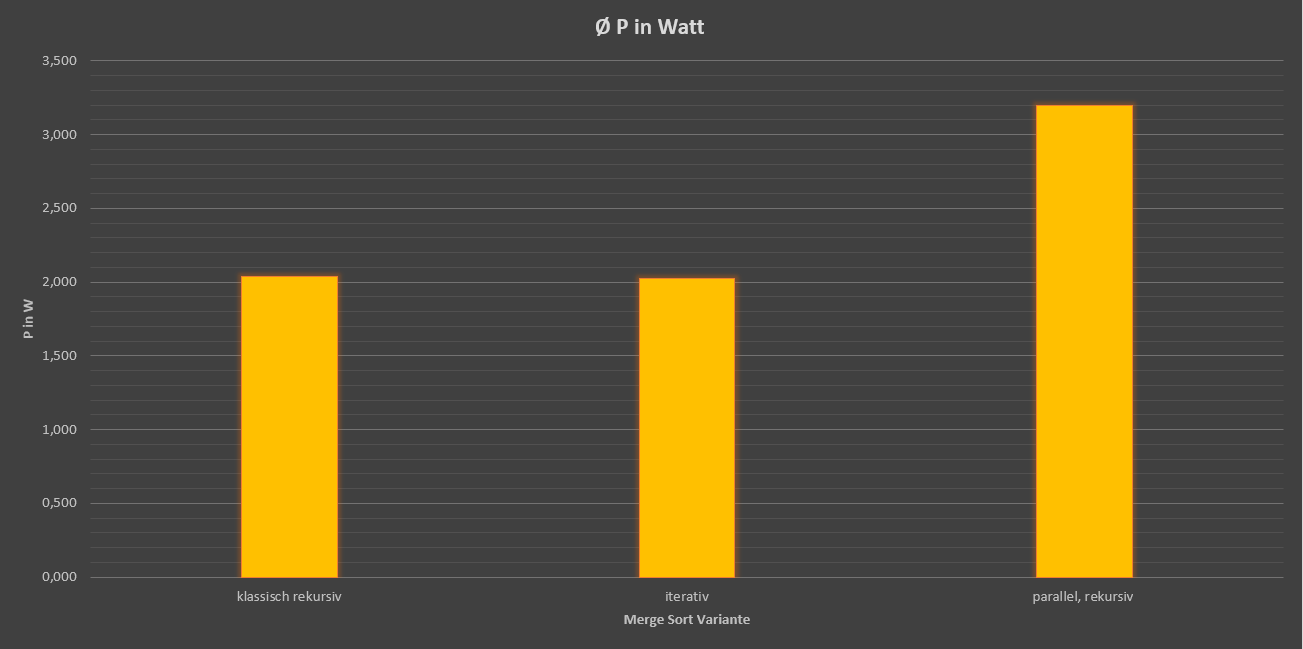
\includegraphics[width=0.8\textwidth]{MergeSortLeistungPic}
	\caption{Merge Sort: durchschnittliche elektrische Leistung pro Verfahren (eigene Abbildung)}
	\label{fig:MergeSortLeistungPic}
	\end{center}
\end{figure}
In \autoref{tab:MergeSortLaufzeitArbeit} ist eine Gegenüberstellung der Laufzeiten und des Energieverbrauchs der verschieden Merge Sort Varianten zu sehen. Die grafische Darstellung erfolgt in \autoref{fig:MergeSortLaufzeitArbeitPic} in einem Balkendiagramm. Da die durchschnittliche Leistungsaufnahme der sequentiell, rekursiven und iterativen Sortierung beinahe identisch ausfällt, ist für den Vergleich der Energieeffizienz der beiden Verfahren die Laufzeit der ausschlaggebende Faktor. So ist die iterative Sortierung mit einer Laufzeit von 714,388 Sekunden ungefähr 11,2 \% schneller als die rekursive  Sortierung. Aufgrund der fast identischen Leistungsaufnahme der beiden Verfahren sinkt auch die verrichtete elektrische Arbeit der iterativen Sortierung um vergleichbare 11,5 \%. Die parallele Sortierung mittels \emph{ForkJoinPool} kann aufgrund der Nutzung von allen Rechenkernen eine deutliche Verringerung der Laufzeit um 41,1 \% vorweisen. Da jedoch die Leistungsaufnahme aufgrund der starken Auslastung der \ac{cpu} während der Ausführung wesentlich höher ist als die der beiden sequentiellen Varianten, ist benötigte elektrische Arbeit nur um 41,1 \% gesunken. Trotzdem ist dies mit Abstand die energieeffizienteste Implementierung.

% Table generated by Excel2LaTeX from sheet 'Tabelle1'
\begin{table}[htbp]
  \centering
  \caption{elektrische Arbeit und Laufzeit der Merge Sort Varianten Gegen\"uberstellung}
    \begin{tabular}{lrr}
    \toprule
    Merge Sort Variante & \multicolumn{1}{l}{t in s} & \multicolumn{1}{l}{W in Ws} \\
    \midrule
    rekursiv & 804,252 & 1662,462 \\
    \midrule
    iterativ & 714,388 & 1471,137 \\
    \midrule
    parallel & 284,021 & 979,787 \\
    \bottomrule
    \end{tabular}%
  \label{tab:MergeSortLaufzeitArbeit}%
\end{table}%


\begin{figure}[H]
	\begin{center}	 
	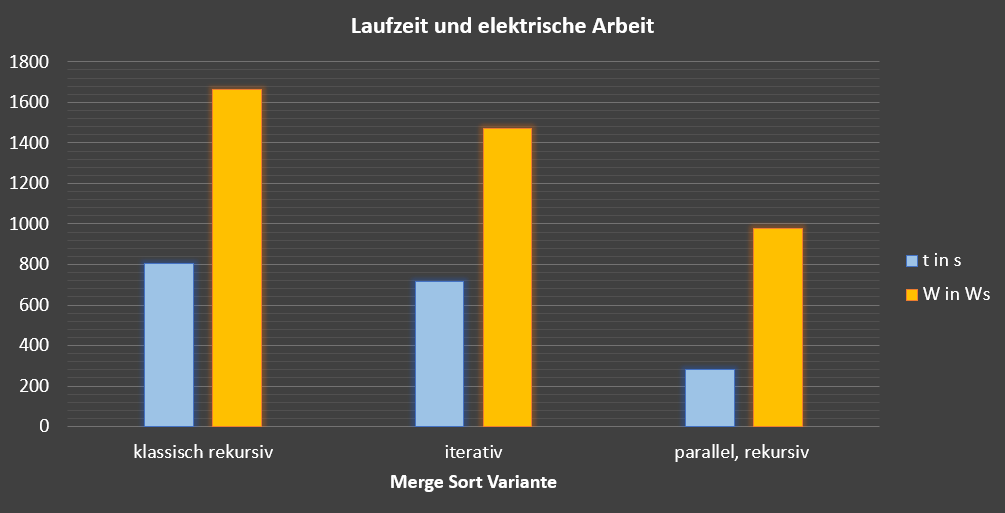
\includegraphics[width=0.8\textwidth]{MergeSortLaufzeitArbeitPic}
	\caption{Merge Sort: Gegenüberstellung von Laufzeiten und elektrischer Arbeit (eigene Abbildung)}
	\label{fig:MergeSortLaufzeitArbeitPic} 
	\end{center}
\end{figure}

\section{Gewonnene Erkenntnisse}

Für die Gegenüberstellung von iterativer und rekursiver Implementierung lässt nach der Betrachtung der Messergebnisse festhalten, dass iterative Implementierungen nicht nur laufzeiteffizienter sind sonder auch energieeffizienter. Dies liegt allerdings nicht an einer höheren Auslastung der \ac{cpu}, welche für iterative und rekursive Implementierungen gleicher Komplexität nahezu identisch ausfällt. Der entscheidende Faktor, ist die erhöhte Laufzeit bei rekursiven Verfahren, welcher mit der stärkeren Belastung des Speichers zu begründen ist. Aufgrund der verschachtelten Funktionsaufrufe bei rekursiven Algorithmen sind wesentlich mehr Speicherzugriffe notwendig. Diese Speicherzugriffe benötigen jedes Mal vergleichsweise viel Zeit und bremsen die Berechnung der \ac{cpu}. Für jeden Funktionsaufruf, muss der entsprechende Overhead des Funktionsaufrufs auf dem Heap des Speichers allokiert werden bevor die eigentliche Berechnung der \ac{cpu} starten kann. Während der Zeit der Allokation, befindet sich die \ac{cpu} im Wartezustand und ist daher nicht optimal ausgelastet. Ein Beweis für diesen Effekt kann die minimal geringere Leistungsaufnahme während der rekursiven Sortierung sein. Dies ist in \autoref{tab:MergeSortLeistung} dargestellt. Die parallele Merge Sort Variante mittels \emph{ForkJoinPool} ist mit Abstand am energiesparendsten. Allerdings muss bei der Implementierung rekursiver Algorithmen mit einem \emph{ForkJoinPool} darauf geachtet werden, dass die Rekursionstiefe sinnvoll begrenzt wird. Da für jede Teilung des Problems (Teile und Herrsche Verfahren) jeweils ein neues Java-Objekt (\emph{RecursiveAction}) erstellt wird, würde eine Zerstückelung der Eingabemenge bis hin zu Mengen mit nur einem Element zu viel Speicher kosten und den Geschwindigkeitsvorteil zunichte machen. Generell sollte daher eine iterative Lösung der Rekursion vorgezogen werden. Besonders im Kontext von mobilen Geräten, da vor Allem der Arbeitsspeicher durch rekursive Algorithmen stärker belastet wird und dies bis heute eine Schwachstelle der mobilen Geräte ist.